\documentclass{article}
\usepackage{cmap} % поиск в PDF
\usepackage[T2A]{fontenc} % кодировка
\usepackage[utf8]{inputenc} % кодировка исходного текста
\usepackage[english,russian]{babel} % локализация и переносы
\usepackage[usenames]{color}
\usepackage{colortbl}
\usepackage{url}
\usepackage{amsfonts}
\usepackage{amsmath}
\usepackage{amsthm}
\usepackage{amssymb}
\usepackage{graphicx} %package to manage images
\graphicspath{{pictures/}}
\theoremstyle{definition}
\DeclareGraphicsExtensions{.pdf,.png,.jpg}
\usepackage[rightcaption]{sidecap}
\usepackage{wrapfig}
\usepackage{ mathrsfs }
\usepackage{indentfirst}
\usepackage{a4wide}
\newcommand{\RNumb}[1]{\uppercase\expandafter{\romannumeral #1\relax}}
\newcommand{\sgn}{\mathop{\mathrm{sgn}}}
\newcommand{\conv}{\mathop{\mathrm{conv}}}


\begin{document}

\thispagestyle{empty}

\begin{center}
\ \vspace{-3cm}

{\scshape Московский государственный\\
Ордена Ленина, Ордена Октябрьской Революции,\\
Ордена Красного Трудового Знамени\\
университет имени М.~В.~Ломоносова}\\
Факультет вычислительной математики и кибернетики\\
Кафедра системного анализа

%\vfill
\vspace{1cm}
\begin{center}
{
\includegraphics[width=6cm]{mgu}}
\end{center}
\vspace{1cm}

{\LARGE Отчёт по практикуму на ЭВМ}

\vspace{1cm}

{\Huge\bfseries <<Решение линейной задачи быстродействия>>}
\end{center}

\vspace{1cm}

\begin{flushright}
  \large
  \textit{Студент 315 группы}\\
  А.\,А.~Самойлов

  \vspace{5mm}

  \textit{Руководитель практикума}\\
  к.ф.-м.н., доцент П.\,А.~Точилин
\end{flushright}

\vspace{5cm}

\begin{center}
  2021
\end{center}

\newpage

\tableofcontents

\newpage

\section{Постановка задачи}
Задана линейная система дифференциальных уравнений:

$\dot x = Ax+Bu+f, ~t \in [t_0, +\infty);~ x,f,u \in \mathbb{R}^2;~
A,B \in \mathbb{R}^{2\times2}$

На значения управляющих параметров u наложено ограничение: $u \in \mathcal{P}$
Пусть $\mathcal{X}_0$ - начальное множество значений фазового вектора, $\mathcal{X}_1$
– целевое множество значений фазового вектора. 
Необходимо решить задачу быстродействия, т.е. найти минимальное время
$T > 0$, за которое траектория системы, выпущенная в момент времени $t_0$ 
из некоторой точки множества $\mathcal{X}_0$, может попасть в некоторую точку множества 
$\mathcal{X}_1$.

$\mathcal{P} = \{x = (x_1,x_2)' \in \mathbb{R}^2: a(x_1-p_1)^4+b(x_2-p_2)^2 \leqslant c\};~
a,b,c > 0$

$\mathcal{X}_1$ --- выпуклая оболочка трех квадратов с длинами сторон $r_1,r_2,r_3$, 
с центрами в точках $x^{(1)}, x^{(2)}, x^{(3)}$
(сторны квадратов параллельны координатным осям);

$\mathcal{X}_1 = \{x_1\}.$

Необходимо написать в среде MatLab программу с пользовательским интерфейсом, которая по
заданным параметрам $A, B, f, t_0, a, b, c, r_1, r_2, r_3,~ x^{(1)}, x^{(2)}, x^{(3)}, x_1$
определяет, разрешима ли задача быстродействия.
Если задача разрешима, то программа должна (приближенно) найти значение
$T$, построить графики компонент оптимального управления, компонент оптимальной траектории,
сопряженных переменных. Программа должна рассчитывать погрешность выполнения условий
трансверсальности для найденной “оптимальной” траектории.
Программа должна давать пользователю возможность постепенно улучшать результаты
расчетов за счет изменения параметров
численного метода и анализа получающихся приближенных результатов.

Замечание. В программе не должно быть перебора по $x(t_0)$.

В соответствующем заданию отчете необходимо привести все теоретические выкладки, сделанные
в ходе решения задачи оптимального управления, привести примеры построенных оптимальных
управлений и траекторий (с иллюстрациями) для различных параметров системы (обязательно для
различных собственных значений матрицы $A$). Необходимо также исследовать на непрерывность
величину $T$ по начальному (целевому) множеству фазовых переменных.

\newpage

\section{Теоретическая база}
\subsection{Немного об опорных функциях}

\textit{Опорная функция} множества $F \in \mathbb{R}^n$ ---
скалярная функция $\rho(l | F)$ векторного аргумента $l \in \mathbb{R}^n$,
определяемая условием $$\rho(l | F) = \sup _{x \in F}{\langle x, l \rangle}.$$

\textit{Важное свойство 1:}

\noindentЕсли $\conv F$ --- выпуклая оболочка множества $F$, то $$\rho(l|\conv F) = \rho(l|F).$$

\textit{Важное свойство 2:}

\noindent$$\rho(l|F \cup G) = \max\{\rho(l|F),~\rho(l,G) \}.$$

\newtheorem{theorem}{Теорема}
 	\begin{theorem}
 		\textit{(Принцип максимума Понтрягина)}

    Пусть допустимое управление $u(t) \in \mathcal{P}, t \in [t_0,t_1]$, переводящее фазову точку из положения 
    $x_0 = x(t_0) \in \mathcal{X_0}$ в положение $x_1 = x(t_1) \in \mathcal{X_1}$, а $x(t)$  --- 
    соответствующая траектори, то есть решение системы при заданном $u(t)$, такое, что $x(t_0) = x_0, x(t_1) = x_1$.
    Для оптимальности по быстродействию управления $u(t)$ и траектории $x(t)$ необходимо существование
    такой ненулевой непрерывной вектор-функции $\psi(t) = (\psi_1(t),\psi_2(t),...,\psi_n(t))'$:

    1) $\dot \psi(t) = -A'(t)\psi(t), \psi(t) \neq 0$,

    2) $\langle \psi(t), B(t)u(t)\rangle = \rho(\psi(t)|B(t)\mathcal{P}(t))$,

    3) $\langle \psi(t_0), x(t_0)\rangle = \rho(\psi(t_0)|\mathcal{X}_0)$,

    4) $\langle - \psi(t_1), x(t_1)\rangle = \rho(-\psi(t_1)|\mathcal{X}_1)$,
	\end{theorem}

\subsection{Опорная функция квадрата}

Опишем множество, которое рассматривается в задаче:
$$\mathcal{S} = \{ \forall z_1, z_2 \in \mathbb{R}^2: \max\{|z_1|, |z_2|\} \leqslant a \}.$$

Для~ее~решения необходимо найти максимум скалярного произведения:
$$\langle \textit{l} , z \rangle = l_1z_1+l_2z_2.$$

Поскольку максимум достигается на~вершинах квадрата,
$$\rho(\textit{l}~|\mathcal{S}) = a(|l_1|+|l_2|).$$

Допустим, что центр квадрата находится не~в~начале координат, а~в~произвольной точке 
$z' = (z_1',z_2')$. Воспользуемся свойством опорной функции и получим:
$$\rho(\textit{l}~|\mathcal{S}+z') = a(|l_1|+|l_2|)
+ \langle \textit{l} , z' \rangle.$$

\subsection{Опорная функция $\mathcal{X}_0$}

$\mathcal{X}_0$ строится как выпуклая оболочка трех квадратов с длинами сторон $r_1, r_2, r_3$ и
центрами в $x^{(1)}, x^{(2)}, x^{(3)}$. Назовем их $\mathcal{S}_i, i = 1,2,3$ соответственно.
Используем \textit{важные свойства 1 и 2}:

$$\rho(l|\mathcal{X}_0) = \rho(l|\conv \bigcup\limits_{i = 1,2,3} \mathcal{S}_i) = 
\rho(l|\bigcup\limits_{i = 1,2,3} \mathcal{S}_i)=$$ $$= \max_{i = 1,2,3} \rho(l|\mathcal{S}_i) = 
\max_{i = 1,2,3} \frac{r_i}{2}(|l_1|+|l_2|) + \langle l , x^{(i)} \rangle.$$

\subsection{Опорная функция $\mathcal{X}_1$}

Поскольку $\mathcal{X}_1 = \{x_1\},~ \rho(l|\mathcal{X}_1) = \langle l, x_1 \rangle.$

Учитывая, что $\mathcal{X}_1$ - точка, а $\mathcal{X}_0$ - выпуклое множество,
удобнее будет решать задачу в обратном времени.
\newpage

\subsection{Опорная функция $\mathcal{P}_0$}

Введем $\mathcal{P}_0 = \{x = (x_1,x_2)' \in \mathbb{R}^2: (x_1)^4+(x_2)^2 \leqslant 1\}$,
предположим, что $l \neq 0$. Полученная задача поиска условного экстремума сводится к 
методу множителей Лагранжа. Определим функцию $\mathcal{L}$:

$$\mathcal{L}(x_1,x_2,\lambda) = x_1l_1+x_2l_2-\lambda(x_1^4+x_2^2-1).$$

Необходимое условие существования условного экстремума - равенство нулю всех
частных производных $\mathcal{L}(x_1,x_2,\lambda)$:

\[
  \begin{cases}
    \frac{\partial \mathcal{L}(x_1,x_2,\lambda)}{\partial x_1} = l_1 - 4\lambda x_1^3 = 0, \\
    \frac{\partial \mathcal{L}(x_1,x_2,\lambda)}{\partial x_2} = l_2 - 2\lambda x_2 = 0, \\
    \frac{\partial \mathcal{L}(x_1,x_2,\lambda)}{\partial \lambda} = -x_1^4-x_2^2+1 = 0.
  \end{cases}
\]

Пусть $l_1 = 0$. Тогда, при решении системы, получим, что $x = (0, \pm 1)'$.
Тогда опорная функция представляется в виде $\rho(l|\mathcal{P}_0) = |l_2|$.
А опорным вектором будет $\psi_0 = (0,\sgn(l_2))'$. 

Пусть $l_2 = 0$. Тогда, при решении системы, получим, что $x = (\pm 1, 0)'$.
Тогда опорная функция представляется в виде $\rho(l|\mathcal{P}_0) = |l_1|$.
А опорным вектором будет $\psi_0 = (\sgn(l_1),0)'$.

Пусть $l_1 \neq 0, l_2 \neq 0$, тогда, $x_1 \neq 0, x_2 \neq 0$. Выразим из первого уравнения 
$\lambda$, из второго уравнения $x_2$ и подставим их в третье уравнение:

\[
  \begin{cases}
    \lambda = \frac{l_1}{4x_1^3}, \\
    x_2 = \frac{l_2}{2\lambda} = 2x_1^3\frac{l_2}{l_1}, \\
    x_1^4 + (2\frac{l_2}{l_1})^2x_1^6 = 1.
  \end{cases}
\]

Рассмотрим функцию $$f_l(t) = (2\frac{l_2}{l_1})^2t^3+t^2-1.$$

Третье уравнение системы эквивалентно уравнению $f_l(x_1^2) = 0$.
Потому начнем искать неотрицательные решения уравнения $f_l(t) = 0$

$f_l(t)$ непрерывна на всей прямой, строго монотонна на
интервале $(0, +\infty)$ и меняет знак на отрезке $[0, 1]$. Значит, на луче $[0, +\infty)$
существует единственное число $\tau_l$ — корень уравнения $f_l(t) = 0$, причем
$\tau_l \in [0, 1]$.
Зная $\tau_l$, можно выписать решение системы:

$$x = \pm (\sqrt{\tau_l}, 2\frac{l_2}{l_1}\sqrt{\tau_l^3})'.$$

Распишем скалярное произведение $\langle x,l \rangle$:

$$\langle x,l \rangle = \pm \sqrt{\tau_l}l_1 \pm 2\frac{l_2}{l_1}\sqrt{\tau_l^3}l_2 = 
\pm l_1^{-1}(\sqrt{\tau_l}l_1^2+2\sqrt{\tau_l^3}l_2^2).$$

Выражение в скобках положительно, и для максимизации скалярного произведения будем брать такой 
знак, чтобы он совпадал со знаком $l_1$. Тогда, для опорной функции $\mathcal{P}_0$ 
справедливо: $$\rho(l|\mathcal{P}_0) = |\sqrt{\tau_l}l_1+2\frac{l_2}{l_1}\sqrt{\tau_l^3}l_2|.$$

Тогда, опорным вектором будет:

$$\psi_0 = \sgn(l_1)(\sqrt{\tau_l}, 2\frac{l_2}{l_1}\sqrt{\tau_l^3}).$$

Итого, получим:

\[
\rho(l|\mathcal{P}_0) = 
  \begin{cases}
    |l_1|+|l_2|,~ & l_1l_2 = 0, \\
    |\sqrt{\tau_l}l_1+2\frac{l_2}{l_1}\sqrt{\tau_l^3}l_2|,~ & l_1l_2 \neq 0;
  \end{cases}
\]

\[
\psi_0 = 
  \begin{cases}
    (\sgn(l_1), \sgn(l_2))',~ & l_1l_2 = 0,\\
    (\sgn(l_1), \sqrt{\tau_l}, 2\frac{l_2}{l_1}\sqrt{\tau_l^3})',~ & l_1l_2 \neq 0.
  \end{cases}
\]

Неизвестным остается лишь $\tau_1$, но его можно найти с любой точностью как единственный
неотрицательный корень уравнения:

$$(2\frac{l_2}{l_1})^2t^3+t^2-1 = 0,~ t \in [0,1].$$

\subsection{Опорная функция $\mathcal{P}$}

Множество $\mathcal{P}$ задается выражением:

$$\mathcal{P} = \{x = (x_1,x_2)' \in \mathbb{R}^2: a(x_1-p_1)^4+b(x_2-p_2)^2 \leqslant c\}.$$

Пусть $$\mathcal{P}_1 = \{x = (x_1,x_2)' \in \mathbb{R}^2: ax_1^4+bx_2^2 \leqslant c \},$$
$$A = \begin{pmatrix} \frac{a}{c}^{-\frac{1}{4}} & 0 \\ 0 & \frac{b}{c}^{-\frac{1}{2}} \end{pmatrix}.$$

$A$ --- самосопряженная матрица.
Покажем, что $A\mathcal{P}_0 = \mathcal{P}_1$:

$$A\mathcal{P}_0 = \{y: y = Ax, x \in \mathcal{P}_0\} = \{y: x = A^-1y \in \mathcal{P}_0 \} =$$
$$=\{y = (y_1,y_2)': ((\frac{a}{c})^\frac{1}{4}y_1, (\frac{b}{c})^\frac{1}{2}y_2)'
\in \mathcal{P}_0 \} =$$
$$=\{y = (y_1,y_2)': ((\frac{a}{c})^\frac{1}{4}y_1 + (\frac{b}{c})^\frac{1}{2}y_2)^2
\leqslant 1 \} =$$
$$= \{y = (y_1,y_2)': ay_1^4+by_2^2 \leqslant c \} = \mathcal{P}_1.$$

Значит, множество $\mathcal{P}$ представимо в виде:
$$\mathcal{P} = \{p\}+\mathcal{P}_1 = \{p\}+A\mathcal{P}_0.$$

Следовательно, опорная функция: 

$$\rho(l|\mathcal{P}) = \langle p, l \rangle + \rho(Al|\mathcal{P}_0) = 
\langle p, l \rangle +
\begin{cases}
    (\frac{a}{c})^\frac{-1}{4}|l_1| + (\frac{b}{c})^\frac{-1}{2}|l_2|,~ l_1l_2 = 0,\\
    |\sqrt{\tau_{Al}}(\frac{a}{c})^\frac{-1}{4}l_1 + 2\frac{l_2^2}{l_1}\sqrt{\tau_{Al}^3}(\frac{a}{c})^\frac{-1}{4}(\frac{b}{c})^{-1}|,~ l_1l_2 \neq 0.
  \end{cases}
$$

Следовательно, опорный вектор:

$$u^* = p + 
\begin{cases}
    ((\frac{a}{c})^\frac{-1}{4}\sgn(l_1), (\frac{b}{c})^\frac{-1}{2}\sgn(l_2))',~ l_1l_2 = 0,\\
    (\sgn(l_1), \sqrt{\tau_{Al}}(\frac{a}{c})^\frac{-1}{4}, 2\frac{l_2}{l_1}\sqrt{\tau_{Al}^3}(\frac{a}{c})^\frac{-1}{4}(\frac{b}{c})^{-1})',~ l_1l_2 \neq 0.
  \end{cases}
$$

$\tau_{Al}$ - неотрицательный корень уравнения:

$$(2\frac{l_2}{l_1}(\frac{a}{c})^\frac{-1}{4}(\frac{b}{c})^\frac{-1}{2})^2t^3+t^2-1 = 0,~ t \in [0,1].$$

\newpage

\subsection{Нахождение $\psi$ аналитическим способом}

Из Принципа Максимума Понтрягина получим систему:

$$
\begin{cases}
  \dot \psi(t) = -A'(t)\psi(t), \\
  \psi(t) \neq 0.
  \end{cases}
$$

Очевидно, это задача Коши из курса обыкновенных дифференциальных уравнений. Выведем аналитически решение для $\psi$.

$$\frac{d\psi(t)}{dt} = -A'\psi(t) \Rightarrow \frac{d\psi(t)}{\psi(t)} = -A'dt$$
$$\Rightarrow \ln\psi = -A't+C^* \Rightarrow \psi(t) = e^{-A't}C$$

У нас есть начальные условия. Используем их для нахождения частного решения.

$$\psi_0 = e^{-A't_0}C \Rightarrow C = e^{A't_0}\psi_0 \Rightarrow \psi(t) = e^{-A't}e^{A't_0}\psi_0$$

Частное решение найдено.

\newpage
\subsection{Алгоритм решения}

\noindent 1) Проверим множества $\mathcal{X}_0, \mathcal{X}_1$ на вырожденность.

\noindent 2) Переберем все направления для $\psi_0$, задав их как $(\sin(\frac{\pi k}{N}), \cos(\frac{\pi k}{N})$.
Подгоним величину $N$ под необходимую точность решения.

\noindent 3) Для каждого из направлений $\psi_0$ зададим аналитически посчитанную функцию $\psi(t)$ и передадим ее в 
ode45() в системе, содержащей помимо этого опорный вектор $u^* = (u_1,u_2)$, вычисленный в 2.6 и матричное уравнение из условия задачи, к 
которое было слегка изменено в связи с решением задачи в обратном времени. 

\noindent 4) Используя ode45() и единый вектор времени, решим численно с использованием имеющейся функции $\psi(t)$
задачу Коши для $x(t)$.

\noindent 5) Анализируем полученные решения, если таковые есть, и выбираем из них решение с минимальным временем.

\noindent 6) Рисуем на графике множества $\mathcal{X}_0, \mathcal{X}_1$, а также траектории:
ту,что является решением, раскрашиваем в зеленый цвет; остальные - в черный. В графиках сопряженных переменных и управлений
сдвигаем время, чтобы начало отсчета было в нуле.

\noindent 7) Погрешность считается по формуле $\delta = |\langle x,\bar \psi \rangle - r|$, где $\bar\psi = \psi/||\psi||; r = \rho(-\psi)$(опорная функция).

\noindent Примечание: во всех построенных графиках разбиение отрезка времени берется по $0.001$c, $N = 100$.

\newpage

\section{Примеры}

\subsection{Пример 1}

Входные параметры: $A = \begin{pmatrix} 0 & 1 \\ -1 & 0\end{pmatrix}, B = \begin{pmatrix} 1 & 0 \\ 0 & 1\end{pmatrix}, 
f = (0, 0), p = (0,0), a = b = c = 1, \mathcal{X}_1~=~(0,0), \mathcal{X}_0$ задается тремя квадрамами с центрами в точке 
$(0, 2)$ и длинами сторон $0.2, 0.4, 2$ соответственно.

В этом примере рассмотрена упрощенная версия задачи,
с начальными условиями, при которых можно было решить задачу аналитически.
Здесь легко заметить ортогональность оптимальной траектории стороне квадрата.
Мое аналитическое решение полностью соответствует полученному численно с помощью Matlab.

Время: 0.0034

Погрешность: 0.061

\begin{center}
{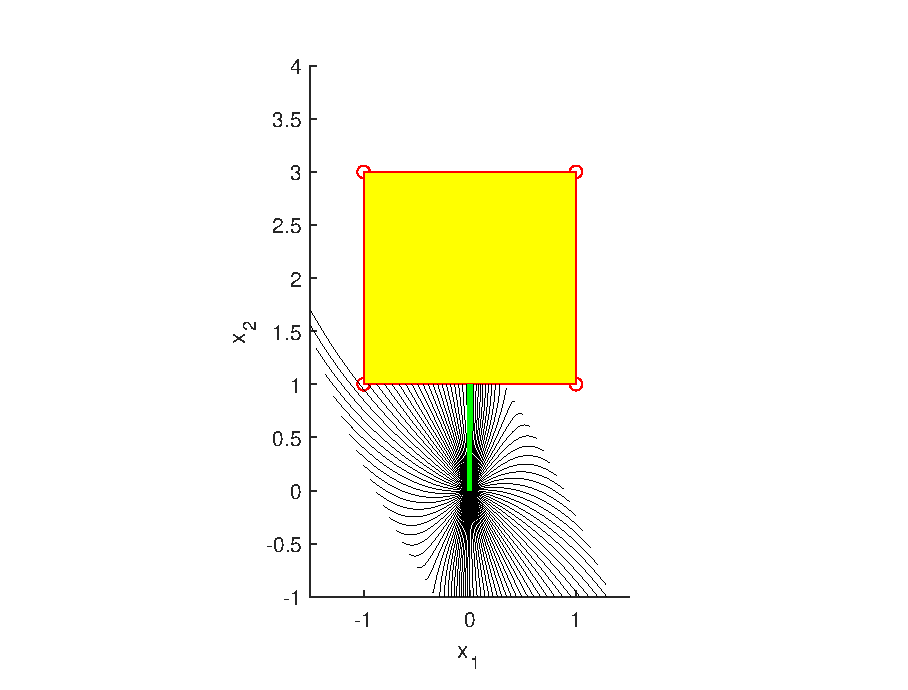
\includegraphics[width=15cm]{example1.eps}}
{Рис. 1. График траекторий}
\end{center}

\begin{center}
  {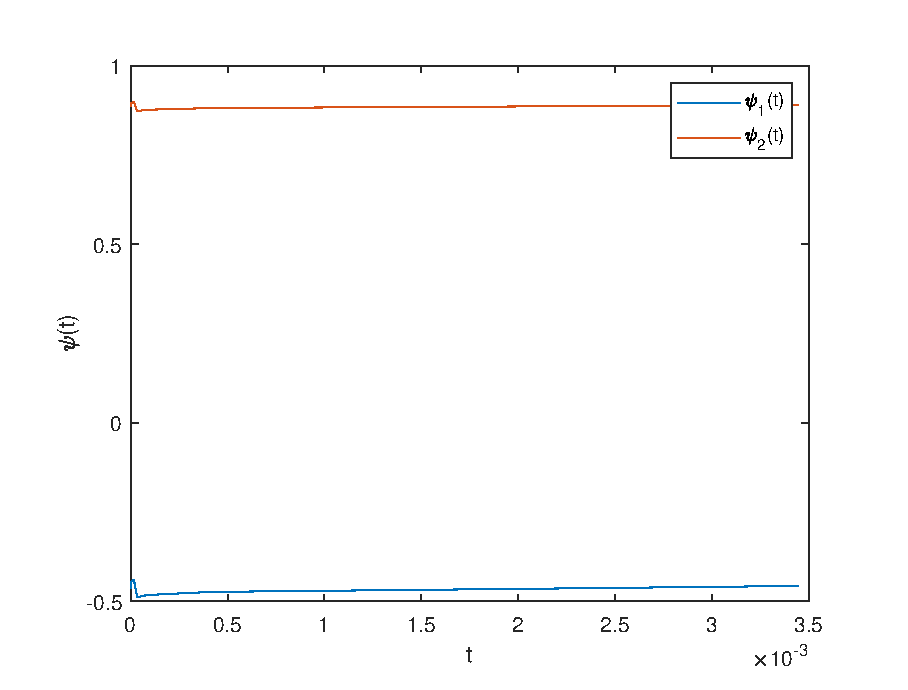
\includegraphics[width=15cm]{pexample1.eps}}
{Рис. 2. График сопряженных переменных}
\end{center}

\begin{center}
  {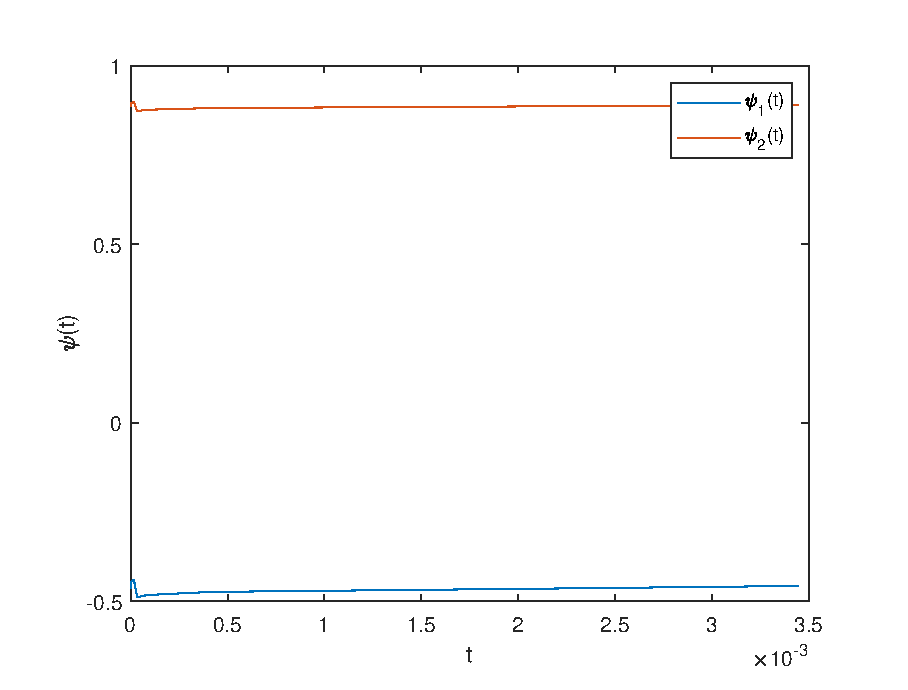
\includegraphics[width=15cm]{uexample1.eps}}
{Рис. 3. График управлений}
\end{center}

\newpage

\subsection{Пример 2}

Входные параметры: $A = \begin{pmatrix} -1 & 10 \\ -5 & 4\end{pmatrix}, B = \begin{pmatrix} 4 & 6 \\ 1 & -7\end{pmatrix}, 
f = (-10, 10), p = (10,-5), a = 2, b = 10, c = 1, \mathcal{X}_1~=~(-8,-6), \mathcal{X}_0$
 задается тремя квадрамами с центрами в точках $(1, -10), (2,3), (3,-4)$,
и длинами сторон $1, 2, 6$ соответственно.

В этом примере можно заметить, что исходное множество (выпуклая оболочка трех квадратов) строится корректно,
также, здесь можно увидеть несмотря на масштабность траекторий на графике, выбранное алгоритмом
оптимальное решение действительно выглядит как кратчайшая траектория, поскольку следует асимптотике растущих функций.

Время: 0.08

Погрешность: 0.036

\begin{center}
{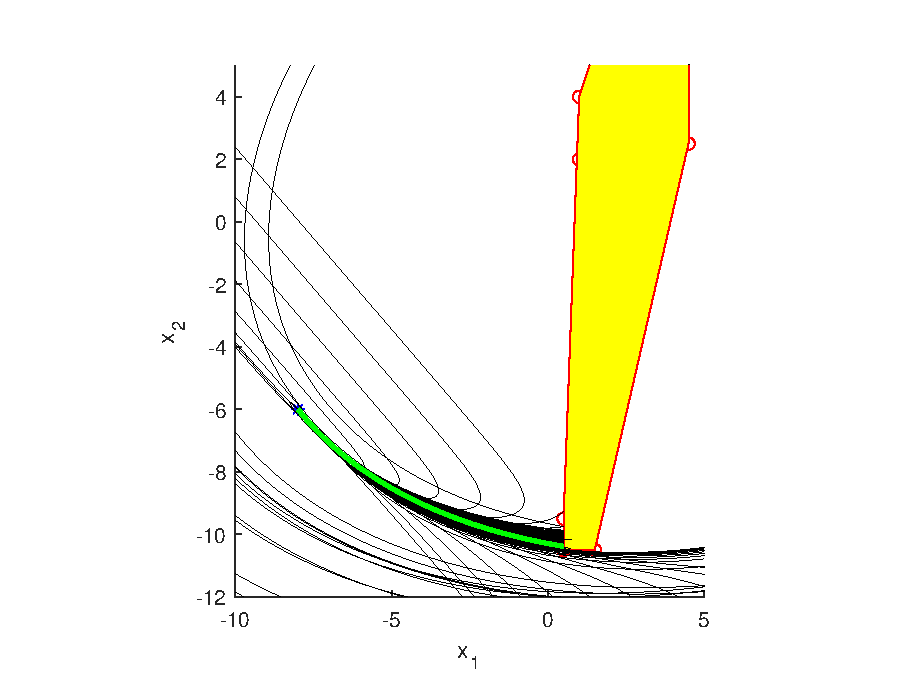
\includegraphics[width=15cm]{example2.eps}}
{Рис. 4. График траекторий}
\end{center}

\begin{center}
{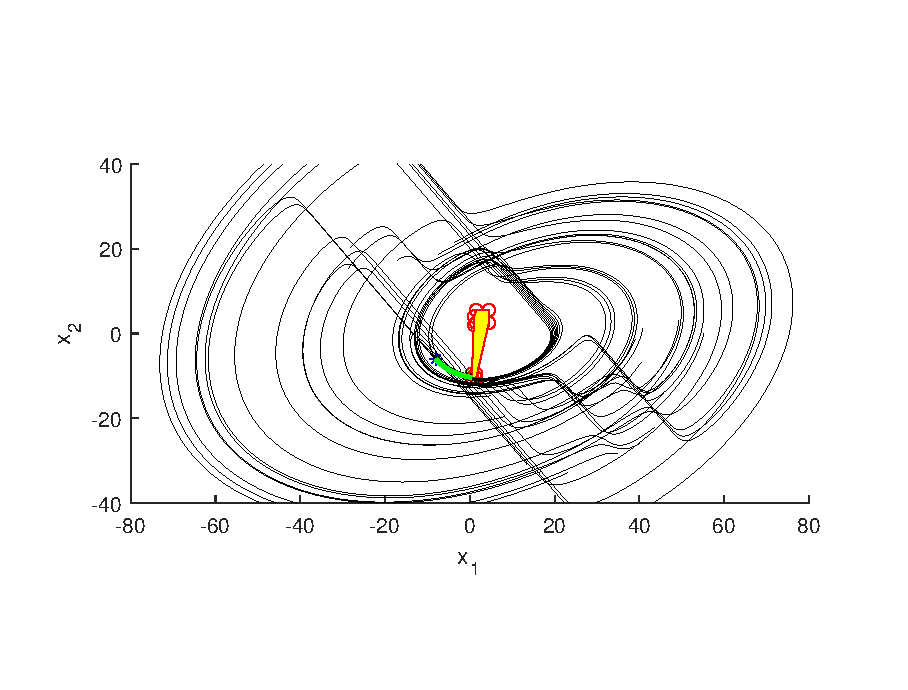
\includegraphics[width=15cm]{example22.eps}}
{Рис. 4.1. График траекторий}
\end{center}

\begin{center}
{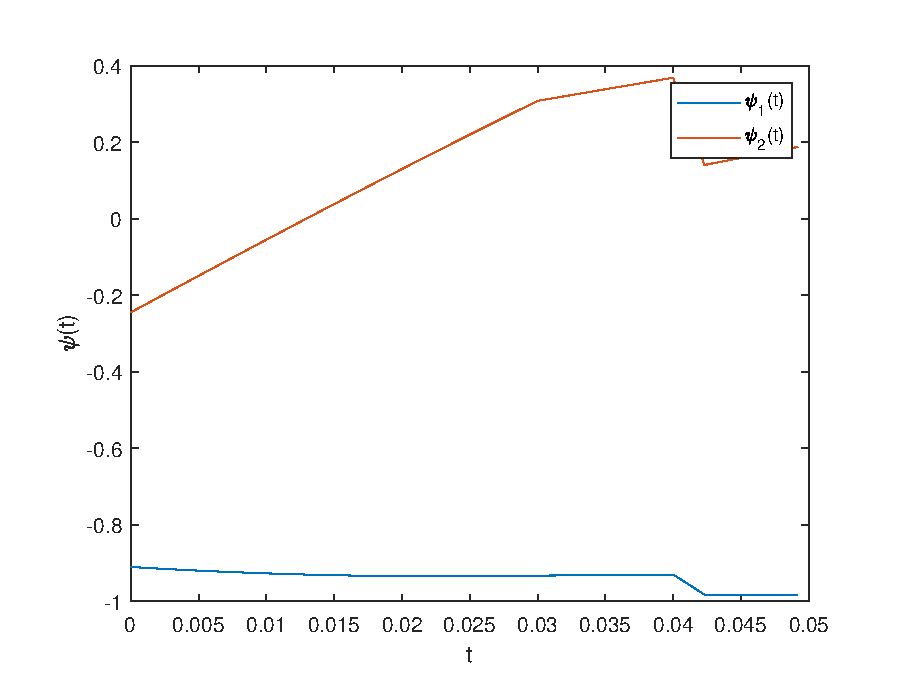
\includegraphics[width=15cm]{pexample2.eps}}
{Рис. 5. График сопряженных переменных}
\end{center}

\begin{center}
  {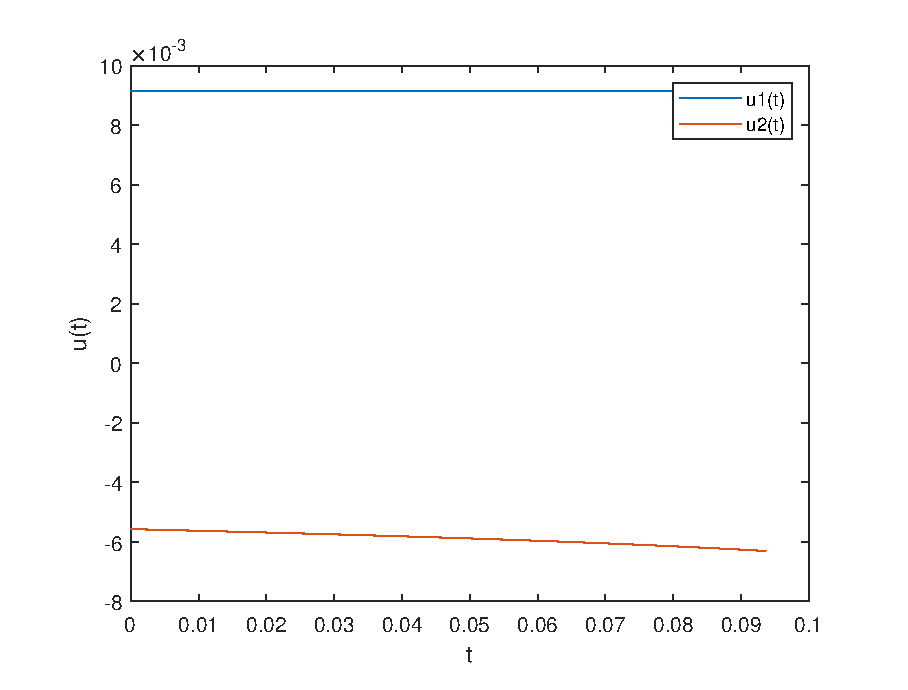
\includegraphics[width=15cm]{uexample2.eps}}
{Рис. 6. График управлений}
\end{center}

\newpage

\subsection{Пример 3}

Входные параметры: $A = \begin{pmatrix} -1 & 20 \\ -5 & 4\end{pmatrix}, B = \begin{pmatrix} 4 & 6 \\ 1 & -7\end{pmatrix}, 
f = (3, 4), p = (10,-5), a = 2, b = 10, c = 1, \mathcal{X}_1~=~(-8,-6), \mathcal{X}_0$
 задается тремя квадрамами с центрами в точках $(1, -10), (2,3), (3,4)$,
и длинами сторон $1, 2, 3$ соответственно.

Этот пример отличается от предыдущего лишь параметром $f$, и можно заметить, как при уменьшении масштаба траекторий, возрастает
кучность решений вокруг оптимального и "чистота" графика: в силу того, что траектории растут медленно, при их попадании в 
множество, они сразу перестают строиться.

Время: 0.034

Погрешность: 0.032

\begin{center}
{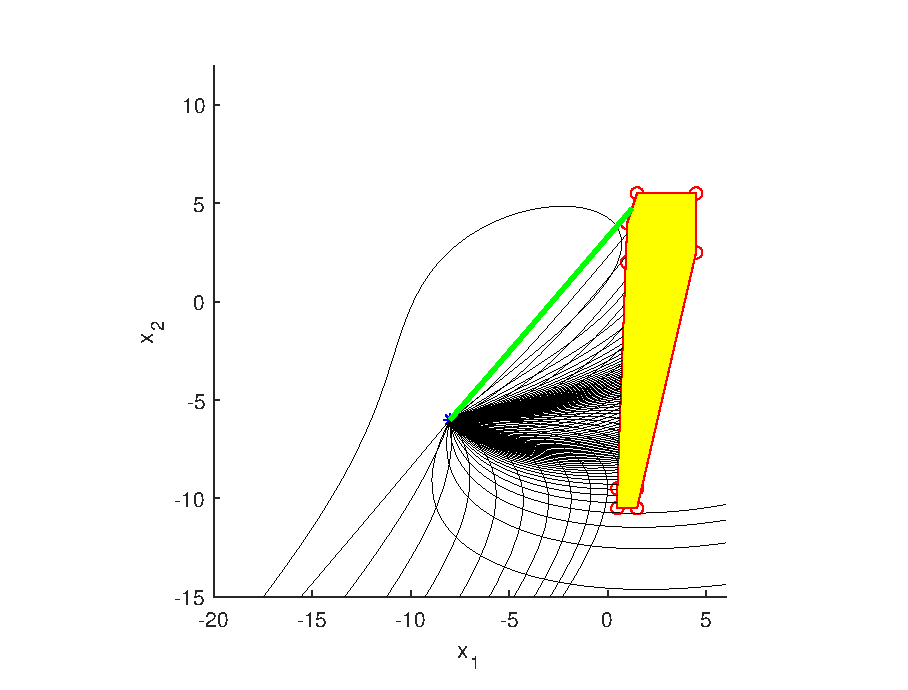
\includegraphics[width=15cm]{example3.eps}}
{Рис. 7. График траекторий}
\end{center}

\begin{center}
{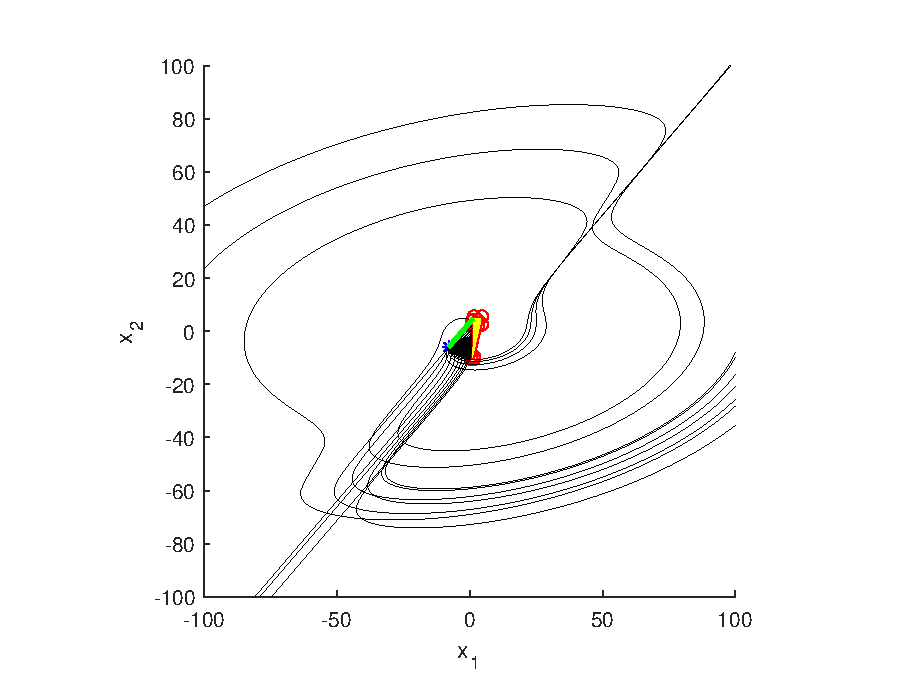
\includegraphics[width=15cm]{example33.eps}}
{Рис. 7.1. График траекторий}
\end{center}

\begin{center}
{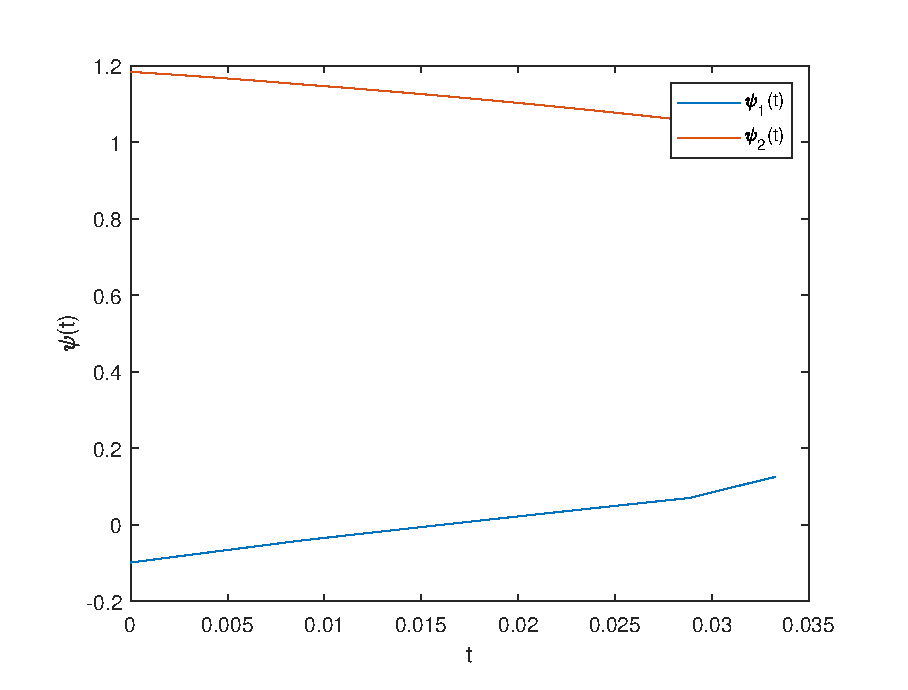
\includegraphics[width=15cm]{pexample3.eps}}
{Рис. 8. График сопряженных переменных}
\end{center}

\begin{center}
{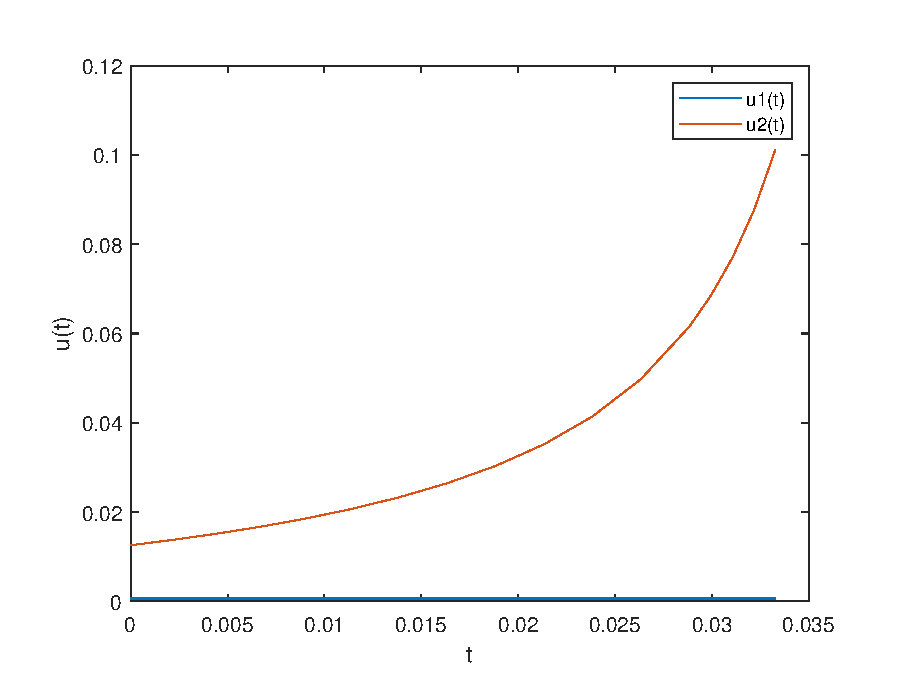
\includegraphics[width=15cm]{uexample3.eps}}
{Рис. 9. График управлений}
\end{center}

\newpage

\subsection{Пример 4}

Входные параметры: $A = \begin{pmatrix} -1 & 20 \\ -5 & 4\end{pmatrix}, B = \begin{pmatrix} 4 & 6 \\ 1 & -7\end{pmatrix}, 
f = (3, 4), p = (0,0), a = 2, b = 10, c = 100, \mathcal{X}_1~=~(-8,-6), \mathcal{X}_0$
 задается тремя квадрамами с центрами в точках $(1, -10), (2,3), (3,4)$,
и длинами сторон $1, 2, 3$ соответственно.

Этот пример отличается от предыдущего параметрами $p, c$, и был на самом деле просто одним из пробных графиков на пути к 
предыдущему примеру. Однако, я оставил его в силу эстетичности получившейся картины.

Время: 0.039

Погрешность: 0.052

\begin{center}
{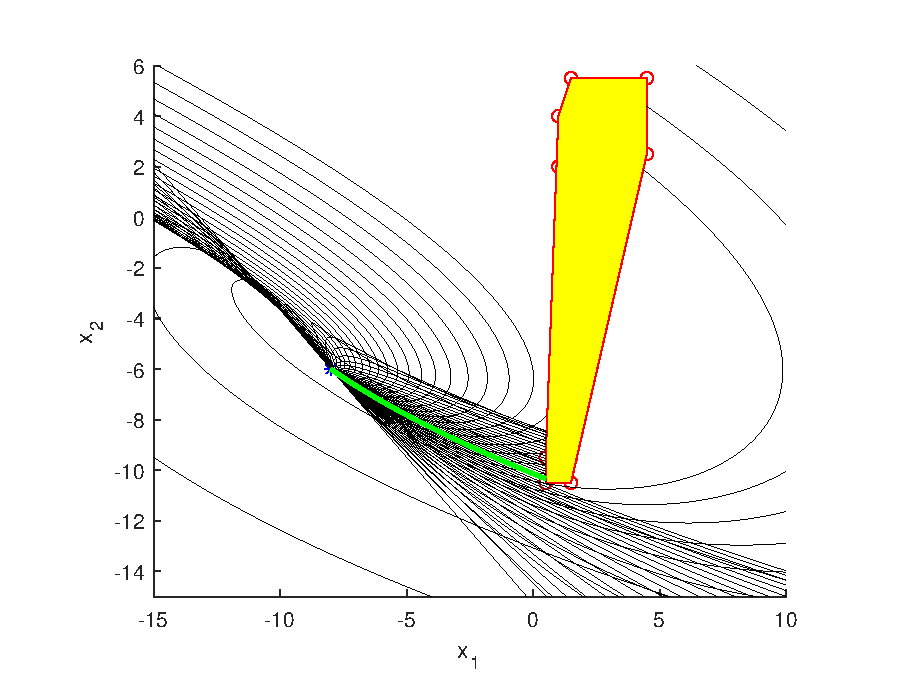
\includegraphics[width=15cm]{example4.eps}}
{Рис. 10. График траекторий}
\end{center}

\begin{center}
{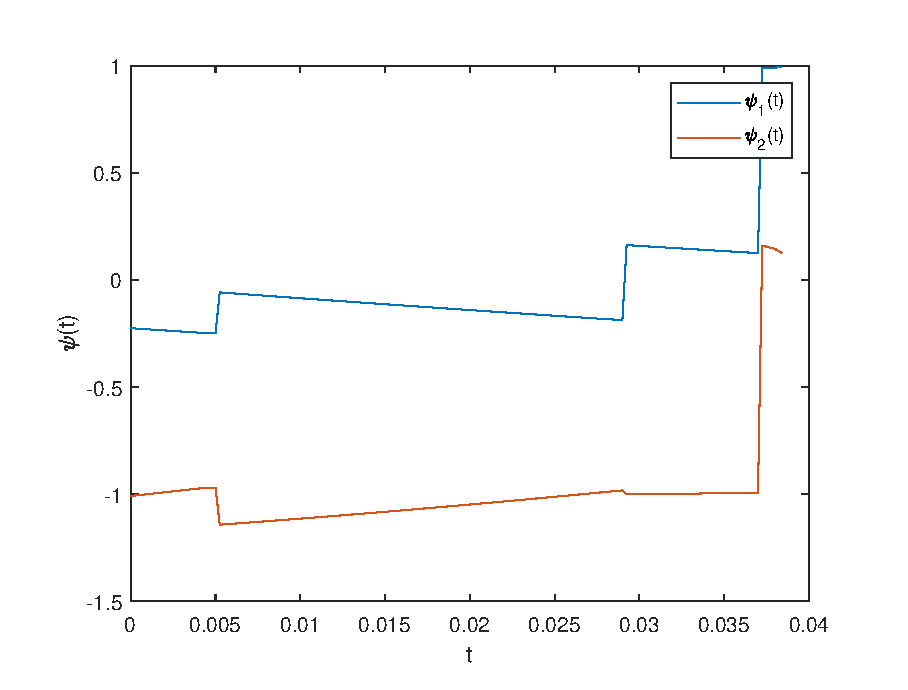
\includegraphics[width=15cm]{pexample4.eps}}
{Рис. 11. График сопряженных переменных}
\end{center}

\begin{center}
{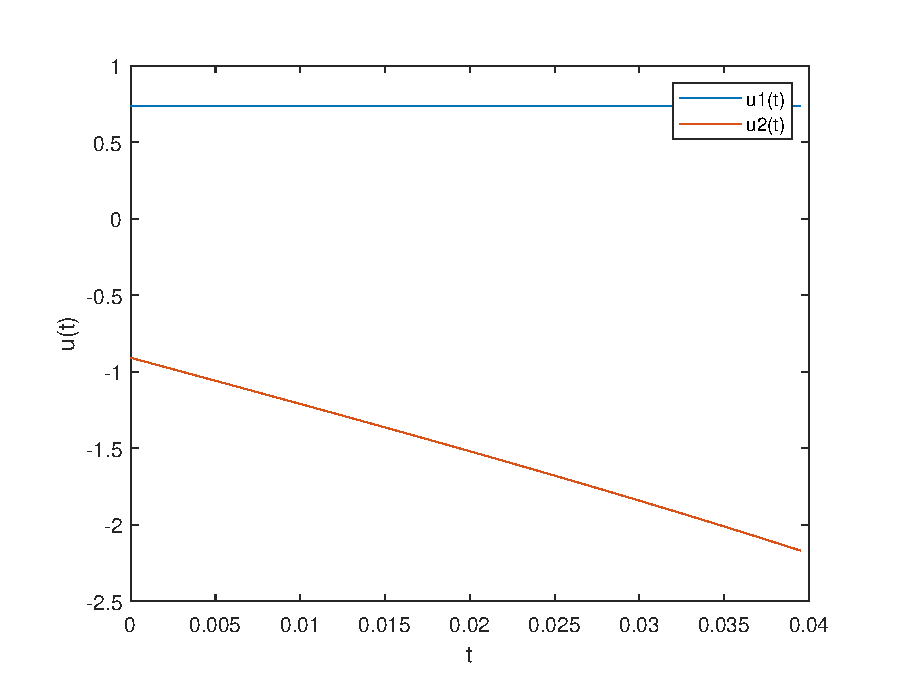
\includegraphics[width=15cm]{uexample4.eps}}
{Рис. 12. График управлений}
\end{center}

\newpage

\subsection{Пример 5}

Входные параметры: $A = \begin{pmatrix} 1 & 2 \\ 3 & 4\end{pmatrix}, B = \begin{pmatrix} 4 & 6 \\ 1 & 7\end{pmatrix}, 
f = (3, 4), p = (0,0), a = 2, b = 10, c = 100, \mathcal{X}_1~=~(-1,1), \mathcal{X}_0$
 задается тремя квадрамами с центрами в точках $(1, 2), (2,3), (3,4)$,
и длинами сторон $1, 2, 3$ соответственно.

Этот пример был включен в отчет по следующим предположениям: на всех предыдущих графиках оптимальное решение почти перпендикулярно
той стороне множества $\mathcal{X}_0$, в которую оно входит. Здесь же наблюдается совершенно иная картина. Причиной тому является
следование траекторий асимптотике некоей прямой на бесконечности. В силу того, что траектории, строимые рядом с этой прямой,
растут быстрее прочих, а $\mathcal{X}_0$ лежит на пути этой прямой, задающей асимптотику, время, полученное для построения
того решения, что видно на графике, действительно является минимальным.

Время: 0.0086

Погрешность: 0.0264

\begin{center}
{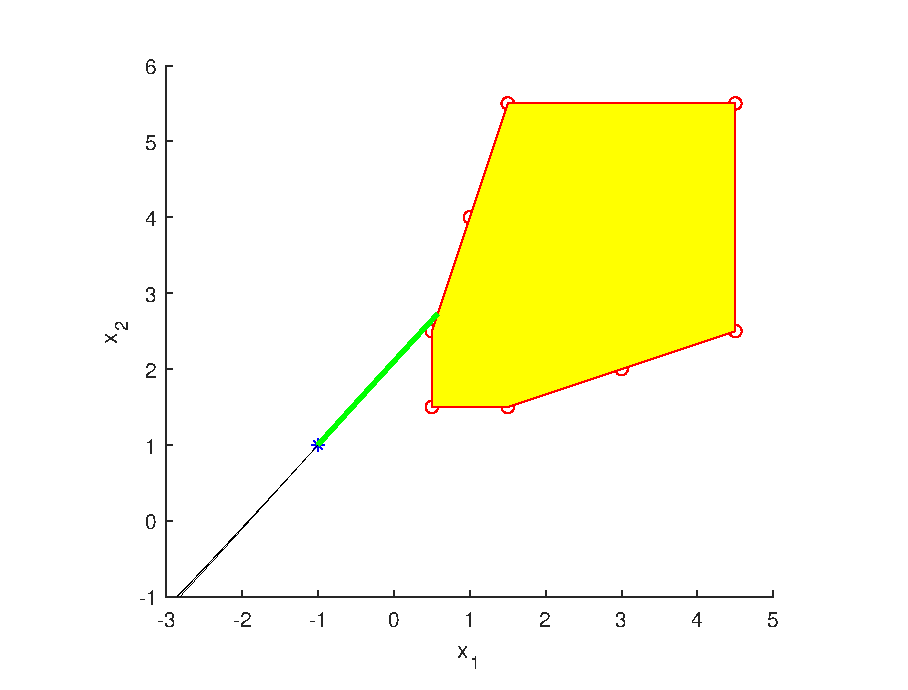
\includegraphics[width=15cm]{example5.eps}}
{Рис. 13. График траекторий}
\end{center}

\begin{center}
{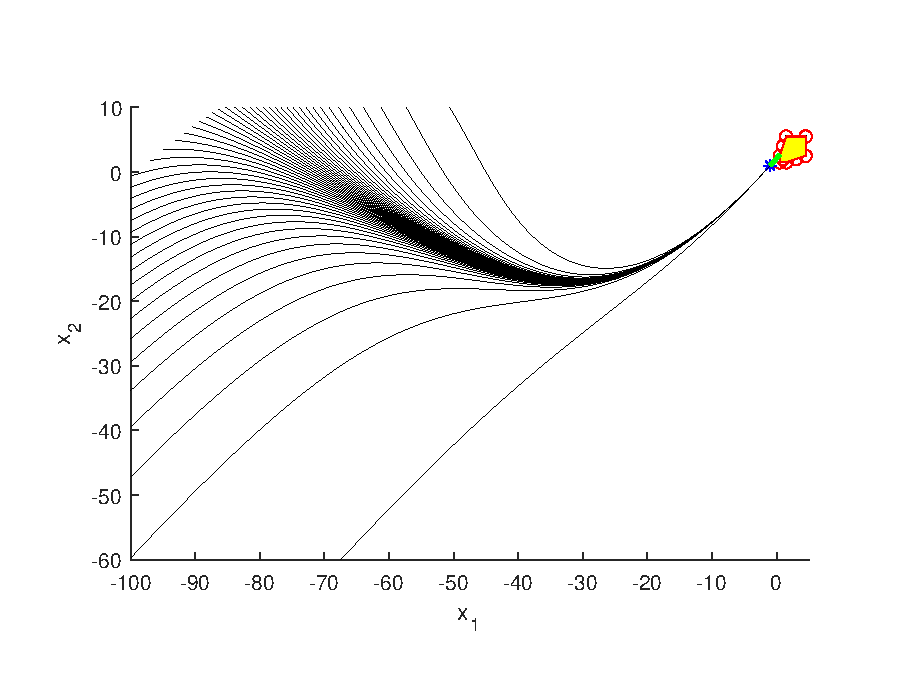
\includegraphics[width=15cm]{example55.eps}}
{Рис. 13.1. График траекторий}
\end{center}

\begin{center}
{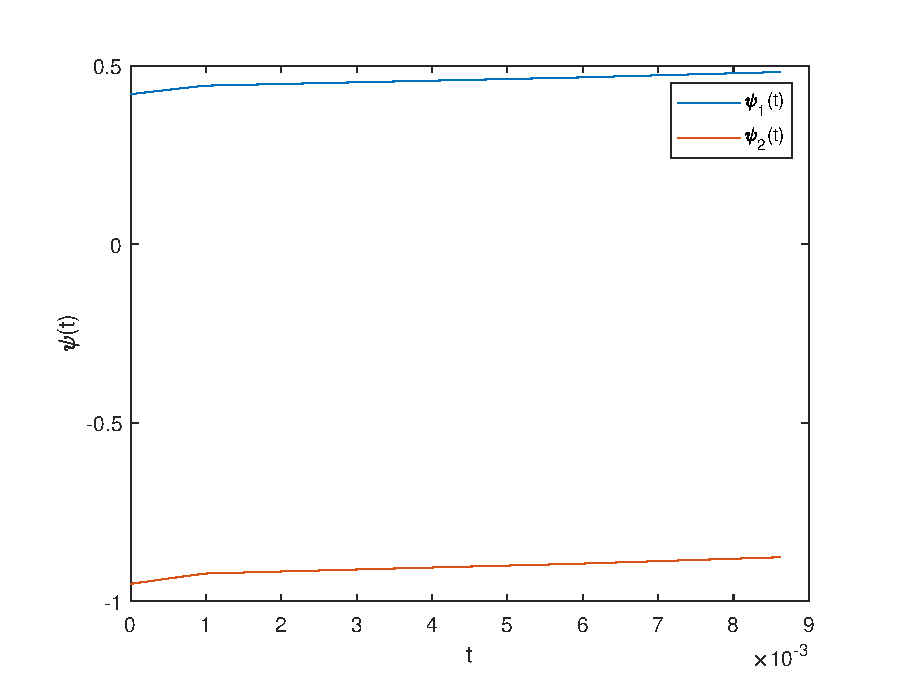
\includegraphics[width=15cm]{pexample5.eps}}
{Рис. 14. График сопряженных переменных}
\end{center}

\begin{center}
{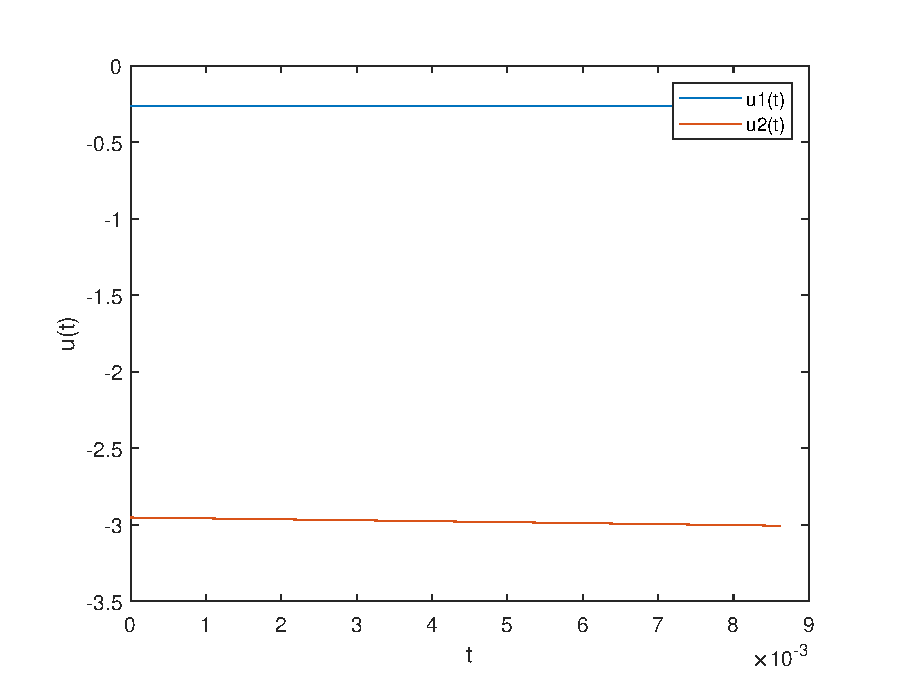
\includegraphics[width=15cm]{uexample5.eps}}
{Рис. 15. График управлений}
\end{center}

\newpage

\subsection{Пример 6}

Входные параметры: $A = \begin{pmatrix} 1 & 2 \\ 3 & 4\end{pmatrix}, B = \begin{pmatrix} 4 & 6 \\ 1 & 7\end{pmatrix}, 
f = (3, 4), p = (0,0), a = 2, b = 10, c = 100, \mathcal{X}_1~=~(-1,1), \mathcal{X}_0$
 задается тремя квадрамами с центрами в точках $(-3, -3), (-2,4), (-1,5.047)$,
и длинами сторон $1, 2, 3$ соответственно.

Данный пример был выбран, чтобы показать, что даже третье число после запятой в координате фигуры может играть большую роль.
У одного из квадратов множества $\mathcal{X}_0$ была выбрана координата $y = 5.047$.
Как можно видеть на графике, траектория едва затрагивает множество.

Время: 0.143

Погрешность: 0.083

\begin{center}
{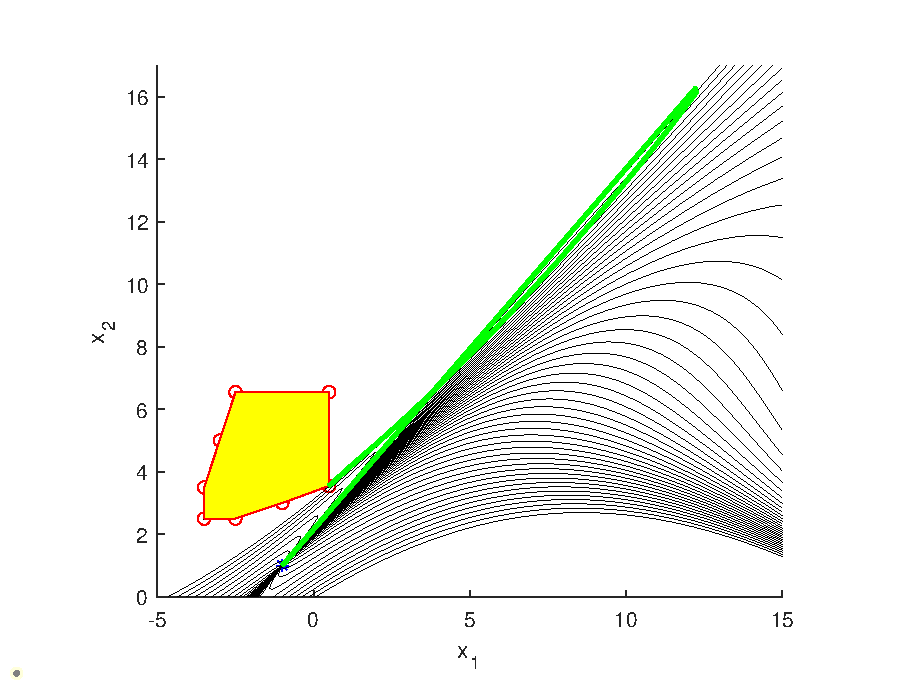
\includegraphics[width=15cm]{example6.eps}}
{Рис. 16. График траекторий}
\end{center}

\begin{center}
{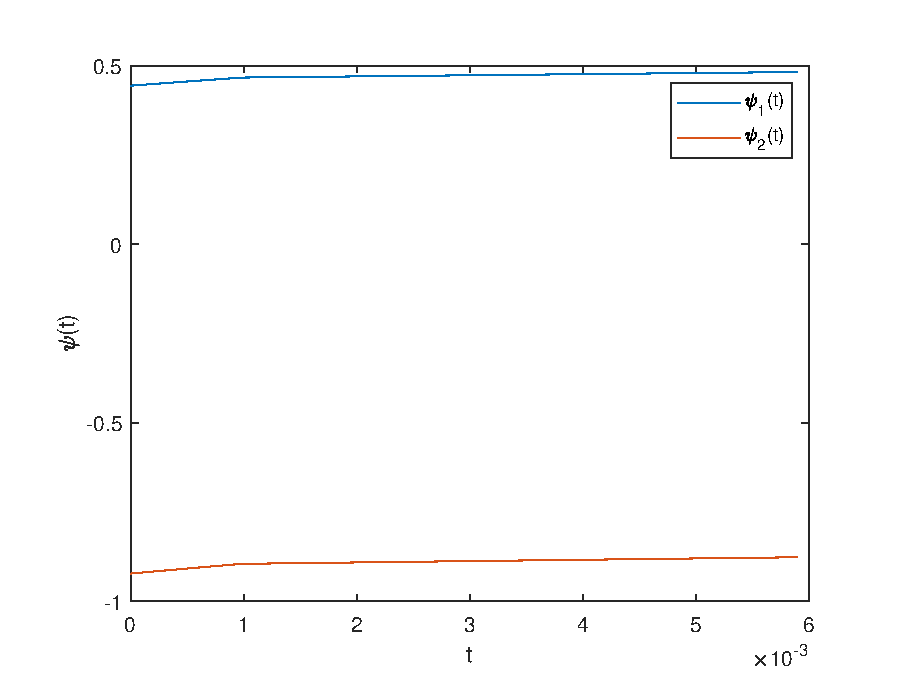
\includegraphics[width=15cm]{pexample6.eps}}
{Рис. 17. График сопряженных переменных}
\end{center}

\begin{center}
{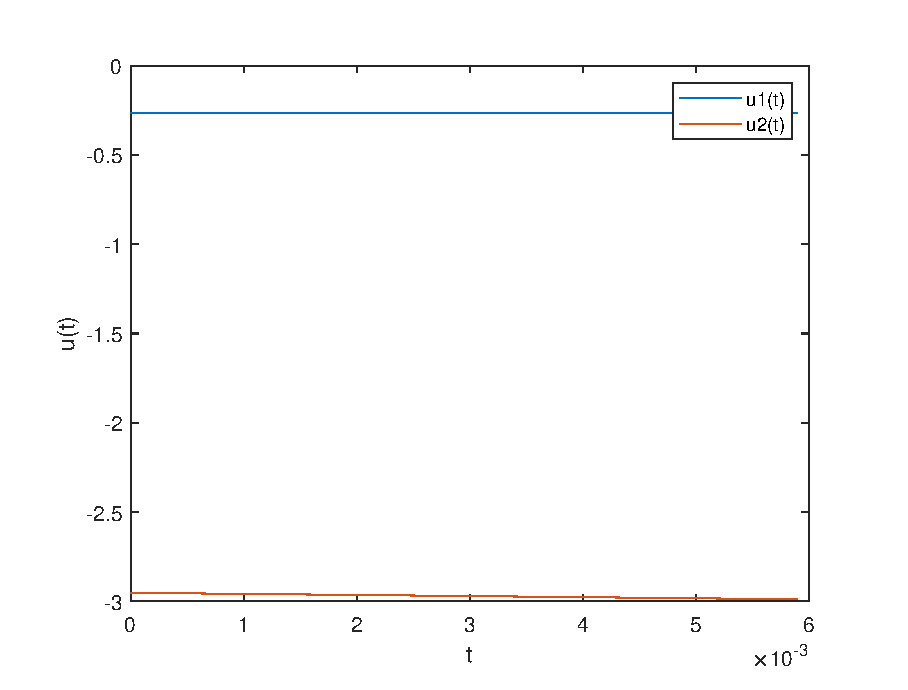
\includegraphics[width=15cm]{uexample6.eps}}
{Рис. 18. График управлений}
\end{center}

\newpage

\subsection{Пример 7}

Входные параметры: $A = \begin{pmatrix} 1 & 2 \\ 3 & 4\end{pmatrix}, B = \begin{pmatrix} 4 & 6 \\ 1 & 7\end{pmatrix}, 
f = (3, 4), p = (0,0), a = 2, b = 10, c = 100, \mathcal{X}_1~=~(-1,1), \mathcal{X}_0$
 задается тремя квадрамами с центрами в точках $(-3, -3), (-2,4), (-1,5.048)$,
и длинами сторон $1, 2, 3$ соответственно.

Данный пример был выбран, чтобы показать, что даже третье число после запятой в координате фигуры может играть большую роль.
У одного из квадратов множества $\mathcal{X}_0$ была выбрана координата $y = 5.048$.
Остальные параметры идентичны тем, что в примере 6.
Как можно видеть на графике, траектория не попадает в множество $\mathcal{X}_0$

\begin{center}
{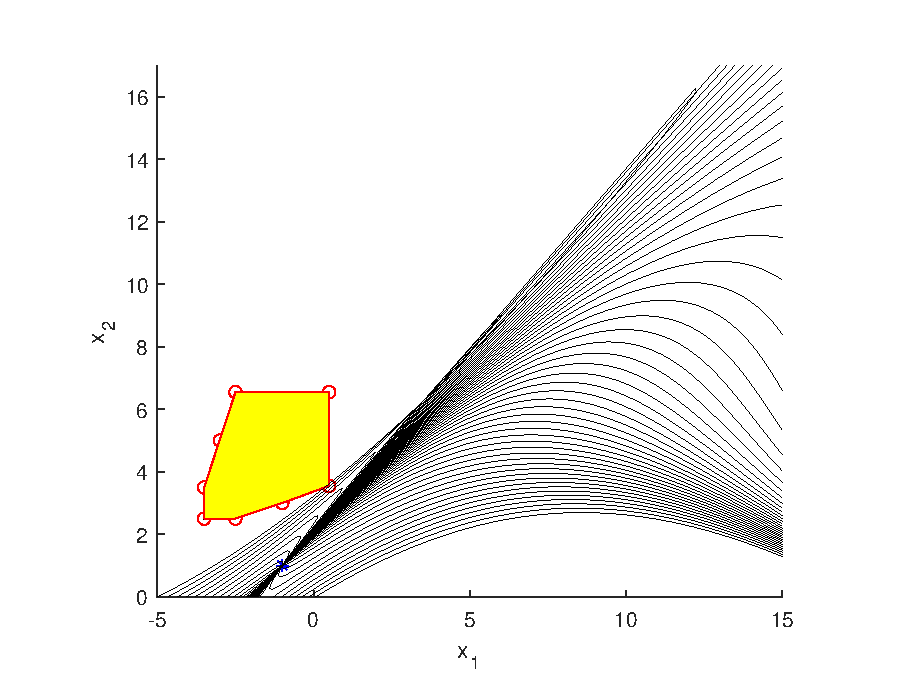
\includegraphics[width=15cm]{example7.eps}}
{Рис. 13. График траекторий}
\end{center}
  

\newpage
\begin{thebibliography}{9}
  \bibitem{lektures} Ли Э.Б., Маркус Л. \emph{Основы теории оптимального управления}.
  \bibitem{OC} Л.С. Понтрягин, В.Г. Болтянский, Р.В. Гамкрелидзе, Е.Ф. Мищенко \emph{Математическая теория оптимальных процессов}.
  \bibitem{lektures} Комаров Ю. \emph{Лекции по курсу оптимальное управление}.
\end{thebibliography}

\end{document}